\documentclass{template/openetcs_article}
\usepackage{graphicx,rotating,color,url}
\graphicspath{{./template/}{./includes/}{.}}

\def\implies{\Rightarrow}

\newcommand{\tbd}{\colorbox{cyan}{\%\%To Be Defined\%\%}}
\newcommand{\tbc}{\colorbox{cyan}{\%\%To Be Confirmed\%\%}}
\newcommand{\todo}[1]{\colorbox{cyan}{\%\%{#1}\%\%}}
\newenvironment{issue}{
	\begin{quote}
	\begin{itshape}Open Issue. 
}{
	\end{itshape}
	\end{quote}
}

\newenvironment{comment}{
	\begin{quote}
	\begin{itshape}Comment. 
}{
	\end{itshape}
	\end{quote}
}

\newenvironment{justif}{
	\begin{quote}
	\begin{itshape}Justification. 
}{
	\end{itshape}
	\end{quote}
}


\begin{document}
\frontmatter
\project{openETCS}
%define your workpackage here
\wp{Work-Package 2: ``Requirements''}

%set a title here
\title{Safety properties for OpenETCS through two examples}

%set a subtitle here



%define a list of authors and their affiliation here

\author{Sylvain Baro\\SNCF}

\affiliation{SNCF INFRA/IG-SYS}
  
  
% define the coverart
\coverart[width=350pt]{chart}

%define the type of report
\reporttype{Note}

\maketitle

\section{Introduction}
Some safety documentation is available in the ERTMS documentation set, despite it has not been 
updated for the Baseline 3.

The SUBSET-88 provides system fault trees, and lists several FMEA documents for various parts 
of the system. The SUBSET-91 summarize the leaves-events of the fault trees, and provides some safety
requirements.

The goal of the current document is to go through some prototyping examples chosen in the document 
\emph{SRS subset for modelling tool benchmarking} and to define on these examples how the Safety 
Requirement could be extracted from the ERTMS documentation downto the model level, and what 
formalism could be used in order to express them.

Please, note that the purpose of the models provided herebelow is not to be completely ``formal''. 
It is only to be sufficiently formal in order to convince oneself that it will be possible to express
executable models and safety properties, and to outline the process followed in order to provide these.

The formalism used for the model is state machines with actions and variables. As for the safety
properties it is a simple propositional calculus which specific predicates to handle transitions 
and states of the model\,\footnote{This is sufficient for the examples in this document, but it 
will probably not be the case for the whole OpenETCS project.}. 

Please also note that the process followed is described in an ``intuitive'' way, in order to make
it easily understandable and to show the different options. This document is not meant to describe 
the Safety Analysis process in a formal way, this should be the purpose of the Safety Plan (WP4). The 
process describe here should only be considered as ``one possible solution''.

\section{Reference documents}
\begin{itemize}
\item WP2/D01 --- \emph{SRS subset for modelling tool benchmarking}
\item SUBSET-026 3.3.0 --- \emph{System Requirement Specification}
\item SUBSET-081 2.3.0 --- \emph{Transmission System: Failure modes and effects analysis}
\item SUBSET-088 2.3.0 --- \emph{ETCS Application Levels 1 \& 2 - Safety Analysis}
\item SUBSET-091 2.5.0 --- \emph{Safety Requirements for the Technical Interoperability
of ETCS in Levels 1 \& 2}
\end{itemize}

\section{Example 1: Establishing a communication session}
In this example, we try to model the requirements in the 3.5.3 section of the SRS SUBSET 26,
for Level 2/3.

The whole purpose of the function is to establish a communication either from the OBU, or from the
RBC. For the sake of simplicity, we will only cover the case where the communication is initiated by 
the OBU.

\subsection{Safety Properties from UNISIG documents}
\label{safety_top}
The processus of identification of the safety properties is a twin process of the processus of 
defining the system and subsystems. 

Once the overall system is defined, the first step for the safety analysis should be to identify 
which are the Safety Properties laying 
on the objects that will be studied and modelled. Usually, in order to defined these Properties,
it is necessary to start at a very high level by the Preliminary Hazard Analysis (PHA) which states the 
system Dread Events for the overall system. These events are very high level: for example we could
find electrocution, or head-on collision.

The overall system should then be split into different subsystem with different area of responsibilities
(for example onboard subsystem, interlocking, driver\dots)

The system-level Dread Events must now be allocated to the different subsystems according to the system
architecture, and refined to 
match the subsystem boundaries and area of responsibilities. This can be done using 
Fault Tree\,\footnote{We will call them Fault Trees even if all events in the trees will not necessarily
be Faults and Failures but could be random or sparse events.} Analysis.

In the case of ERTMS, SUBSET-88 provides such Fault Trees. Fig. \ref{fig:ch_fault_tree} describes for
example the events leading to the Dread Event ``Brake Control Function Failure\,\footnote{Event
if this does not go up to the main system Dread Events, one can easily imagine how this 
could cause a collision}''. The main event is then refined to leaves or other sub-Fault Trees, 
in particular the Tree identified by GATE80, corresponding to an incorrect determination of the 
current mode. 

This mid-level event is then also refined (Fig. \ref{fig:mode_fault_tree}) to events and especially 
leaves that are expected to be of the SRS level. This leads in particular to the lower-level events
KERNEL-3 to KERNEL-6 (see Fig. \ref{fig:mode_fault_tree} or \ref{tab:kernel_evt}) which are related 
to the radio transmission. These lower level events are 
summarized into the SUBSET-91 document, which is a mandatory part of the ERTMS documentation.

\begin{figure}
  \centering
  {For IPR reason, the figure was removed. \\
  The reader shoud refer to SUBSET-88-2 Part 1, Appendix B, p. 2}
  \caption{Core Hazard Fault Tree (SUBSET-88)}
  \label{fig:ch_fault_tree}
\end{figure}

\begin{figure}
  \centering
  {For IPR reason, the figure was removed. \\
  The reader shoud refer to SUBSET-88-2 Part 1, Appendix B, p. 8}
  \caption{Incorrect Mode Fault Tree (SUBSET-88)}
  \label{fig:mode_fault_tree}
\end{figure}

\begin{issue}
Should the Fault Trees Analysis provided in the SUBSET-88 be considered as complete? My feeling is 
that it is not the case, because there is no ERTMS Safety Plan (AFAIK) to track the way the analysis 
was conducted, so there is no proof that the analysis is sufficiently rigorous.

Moreover, we'll see in Sect. \ref{gaps} that the trees should be refined again before being at the proper
level.
\end{issue}

It is now necessary to analyze if each scenario is covered and how (and if the coverage is sufficient).
We will call ``scenario'' the succession of events needed to provoke a studied Dread Event (which could
be high- or low-level). Covering the scenario could be done by proving that a requested leaf is always 
impossible to meet, or by proving that the conjunction of all the requested sub-events would be rarer 
than the THR (Tolerable Hazard Rate) requested for ERTMS application or its allocation to the studied 
sub-system.

%\begin{sidewaysfigure}
\begin{figure}
  \centering
  {For IPR reason, the figure was removed. \\
  The reader shoud refer to SUBSET-88-2 Part 2, p. 23-24}
  \caption{Kernel Dread Events (as in SUBSET-88 or SUBSET-91)}
\label{tab:kernel_evt}
\end{figure}
%\end{sidewaysfigure}

SUBSET-88 provides the following informations on the events that interest us 
(cf. Fig. \ref{tab:kernel_evt}). This table lists the base events (leaves) of the tree
and describes the impact of such events, and the mitigation used to avoid safety problems.
The problem is that whether there is a safety issue is not made that explicit: if we take
KERNEL-6, for example, the description states that a loss of communication could lead either to a 
failure to receive more restrictive route information, or to the driver being obliged to use a lower 
level. We can imagine that these are not catastrophic consequences (we wouldn't risk the safety on 
the probability that a message does not reach its destination), but in order to make this statement,
it needs a system-level analysis. 

Nevertheless, in this case the third part of SUBSET-88 (9.3.3.1) provides an answer \footnote{
The same explanation may be found also in SUBSET-91.}:
\begin{quote}
As indicated in 9.2.2.1, the data exchange between track and train is defined in the
ETCS specifications such that normally the deletion of a message does not result in a
hazard. Moreover, deletion of critical messages is mitigated by means of
acknowledgement procedures. The only case where deletion may lead to a hazardous
situation is in the case of Emergency messages and this situation is considered in the
following section. On the basis of these further considerations the possibility of
undetected deletion of messages is not carried forward as a provable / testable target.
\end{quote}

\begin{issue}
Is it in our scope to provide the analysis stating that message deletion never leads to 
an unsafe situation?
\end{issue}

In the case of KERNEL-4, on the other hand, the situation is clearer. The table states that 
``Radio link supervision'' is a protective function against this event. Hence it is here easy to
determine a safety property for the corresponding function!

In the particular case of the transmission, there is yet another document that provides 
information on safety issue: SUBSET-81 ``FMEA for Transmission System''. We see for the 
line 5.2.4.2 (Fig. \ref{fig:fmea}) that some of the mitigations of the consequences of the loss
of message lie in the transmission protocol, but also in the way of using/dimensionning ERTMS,
which should consider (at a system-level) the impact of the loss of messages.

\begin{figure}
  \centering
  {For IPR reason, the figure was removed. \\
  The reader shoud refer to SUBSET-81-2, p. 15}
  \caption{Part of the FMEA for Transmission System (SUBSET-81)}
  \label{fig:fmea}
\end{figure}

\subsection{Model of the function}
The (simplified) proposed model for the function is provided Fig. \ref{fig:establish_tab} and 
\ref{fig:establish}. The transitions and actions are the following. It is not useful here to detail
more the actions and formalism.

\begin{figure}
\centering
\small
\begin{tabular}{|l|l||p{3.5cm}|p{3.5cm}|}
\hline
\bf From & \bf To & \bf Condition & \bf Action \\
\hline
NoCom & Trying & Order(RBC\_ID) received & RBC\_Com := RBC\_ID \\
\hline
Trying & Trying & No connexion setup & Req. setup of connexion to RBC\_ID \\
\hline
Trying & Setup & Connexion setup & Send Initiation Msg \\
\hline
Setup & NoCom & Received System\_Version(RBC\_ID,V) and not compat(V)  & Disconnect\\
\hline
Setup & Established & Received System\_Version(RBC\_ID,V) and compat(V) & 
		Send Estab. report; V\_Com := V  \\
\hline
\dots & \dots & \dots & \dots  \\
\hline
\end{tabular}
\normalsize
\caption{Establish a communication session (transitions)}
\label{fig:establish_tab}
\end{figure}

\begin{figure}
  \centering
  %  dot establish.dot -Teps -o establish.eps &&  epspdf  establish.eps 
  \fbox{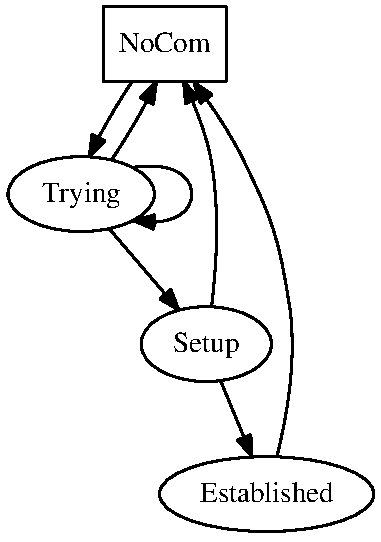
\includegraphics[scale=0.70]{establish.pdf}}
  \caption{Establish a communication session}
  \label{fig:establish}
\end{figure}

\subsection{Safety properties}
If we try to infer some safety properties from this state machine, in a \emph{bottom-up} way 
(rather than the \emph{top-down} way presented in Sect. \ref{safety_top}) we can identify 
a few possible failures. A process to be used in order to find out these events could be
to build a system FMECA starting from the formal model.
\begin{itemize}
\item Not being able to establish a communication while required;
\item Establishing a communication while not required;
\item Establishing a communication with the wrong RBC;
\item Establishing a communication with an incompatible version RBC;
\item \dots ?
\end{itemize}

Considering the events studied in Sect. \ref{safety_top}, we can state that the first item does 
not lead to an unsafe state. It will not yield a safety property. As for the second, the safety status 
is not as clear. It is necessary to conduct a system safety analysis in order to decide if failure 
leads to an unsafe state, and in this cas to state a property to cover this event
(for the sake of brevity, we will not do it in this document). As for the third event, we will consider
it as unsafe, because if we cannot guarantee that the same RBC is used during the whole process, it is 
unlikely that we will be able to perform the version control requested to cover the lattest issue.
The last failure (establishing a communication with an incompatible version
RBC) could clearly lead to an unsafe state, if possible (although a system-level analysis should 
confirm this).

Assuming these are all the safety event we have to cover, we could therefore provide the following 
property in order to cover them. This property is somehow redundant with the model, but it is restricted
to the bare safety need.
$$State = Established \Rightarrow compat(V\_Com)\wedge RBC\_ID = RBC\_Com$$

\subsection{Filling the gaps\dots}
\label{gaps}
If we compare the events provided by the Fault Trees (KERNEL-\emph{xx}) it is clear that they are 
still too high level to be able to be used to build directly the safety properties on the studied 
function. These properties are still high level compared to the degree of description in the SRS. This 
is due to the fact that these events are \emph{functional} although the function studied (establishing
a communication) is a rather low level service.

The question is ``would it be possible to go \emph{formally} from the high level Dread Events to 
the properties which goes on the same level than the model?'' In my opinion this is not practically 
feasible. It would need a very high level model of the system (much higher than the SRS) without any 
allocation to the different subsystem. It would also be necessary to introduce a sufficiently wide 
notion of environment to be able to formalize that communicating with an improper version of software 
could lead to an unsafe behavior.

\begin{figure}
  \centering
  \fbox{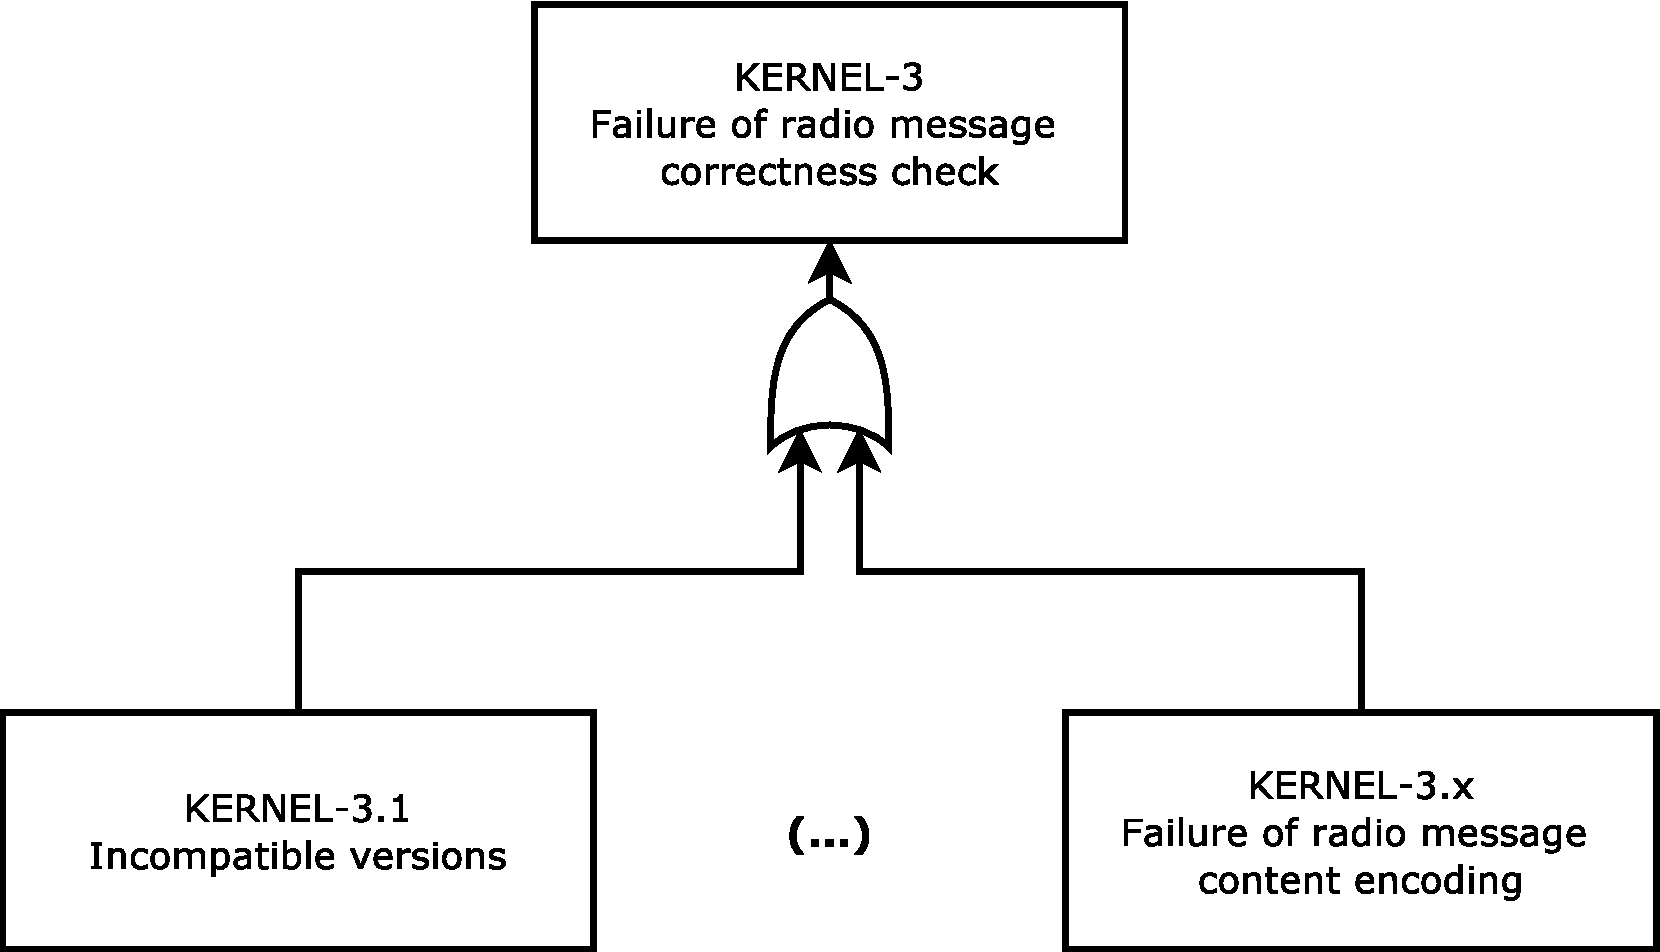
\includegraphics[scale=0.40]{ext_fta.pdf}}
  \caption{Extending the Fault Tree}
  \label{fig:ext_fta}
\end{figure}

It is therefore necessary to conduct a system-level ``brain, paper and pen'' safety analysis to 
be able to build the safety properties on the proper level with regard to a model of the SRS. This
analysis could be carried out either with a \emph{top-down} analysis (cf. Fig. \ref{fig:ext_fta}) or 
by a \emph{bottom-up} analysis (\emph{e.g.} FMECA), or by combining both approaches. It is important
to point out that whichever is the followed method, it is the level of expertise of the safety analyst
above everything else that will guarantee that no unsafe case have been forgotten.

\section{Example 2: Mode Transitions}
The purpose is to modelize some of the mode transitions of the SUBSET-26 4.6.2 table (mode transitions), 
namely the transitions from SB to SH, FS and IS.

\subsection{Model of the function}
The model here is very simple (Fig. \ref{fig:trans_sb_tab} and \ref{fig:trans_sb} ) 
because we do not want to dive into the condition details.

\begin{figure}
\centering
\small
\begin{tabular}{|l|l||p{3.5cm}|p{3.5cm}|}
\hline
\bf From & \bf To & \bf Condition & \bf Action \\
\hline
SB & IS & Isolated &  \\
\hline
SB & FS & FS conditions and not Isolated &  \\
\hline
SB & SH & SH conditions and not Isolated &  \\
\hline
\end{tabular}
\normalsize
\caption{Mode transitions from SB to SH, FS and IS (transitions)}
\label{fig:trans_sb_tab}
\end{figure}

\begin{figure}
  \centering
  %  dot trans_sb.dot -Teps -o trans_sb.eps &&  epspdf  trans_sb.eps
  \fbox{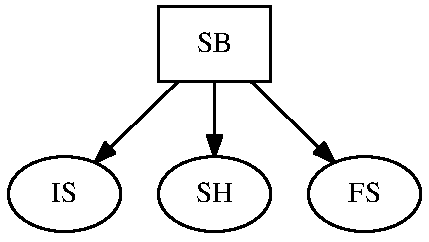
\includegraphics[scale=0.70]{trans_sb.pdf}}
  \caption{Mode transitions from SB to SH, FS and IS}
  \label{fig:trans_sb}
\end{figure}

\subsection{Safety properties}
As for the safety properties, the SUBSET-88 provides the following event. 
\begin{center}
GATE80: Incorrect determination of the current mode
\end{center}
Without a clear hierarchy of modes stating that being in one given mode instead of other ones, we 
shall consider that as far as safety is concerned, a transition must occur if and only if the 
corresponding conditions are verified at the time of the transition.

We do not want to define here a complicated formalism. We use simple predicates
$State(X)$ to write that the machine is in the state $X$, and $A\rightarrow B$ that the machine triggers
a transition from state $A$ to state $B$. The important thing here is that we are introducing some 
dynamic behavior (although we keep on using proposition calculus).

% $$SB\rightarrow IS \iff Isolated\_by\_Driver \wedge State(SB)$$
% $$SB\rightarrow FS \iff FS\_Conditions \wedge \neg Isolated \wedge State(SB)$$
% $$SB\rightarrow SH \iff SH\_Conditions \wedge \neg Isolated \wedge State(SB)$$

$$SB\rightarrow IS \implies Isolated\_by\_Driver$$
$$Isolated\_by\_Driver \wedge State(SB) \implies SB\rightarrow IS$$
$$SB\rightarrow FS \implies FS\_Conditions \wedge \neg Isolated$$
$$FS\_Conditions \wedge \neg Isolated \wedge State(SB) \implies SB\rightarrow FS$$
$$SB\rightarrow SH \implies SH\_Conditions \wedge \neg Isolated$$
$$SH\_Conditions \wedge \neg Isolated \wedge State(SB) \implies SB\rightarrow SH $$

These properties are a bit disappointing, because they are a mere paraphrasing of the state machine
provided in the model. We could try to go a little bit further with a system-level analysis of the 
SUBSET-26 mode transition table. We would like to provide in the safety properties the conditions
which are really relevant to safety (but these might as well be \emph{all}).

For this task we need to consider the transition out of the states. 
For the sake of brevity, we consider only the four modes IS, FS, SB and SH (but we use the full sub-state
machine of the real ETCS mode with these modes) and do not discriminate here the different Shunting 
conditions depending of if the initial state is FS or SB (Fig. \ref{fig:trans_whole} and \ref{fig:trans_whole}).

\begin{figure}
 \centering
\small
\begin{tabular}{|l|l||p{3.5cm}|p{3.5cm}|}
\hline
\bf From & \bf To & \bf Condition & \bf Action \\
\hline
SB & IS & Isolated &  \\
\hline
SH & IS & Isolated &  \\
\hline
FS & IS & Isolated &  \\
\hline
SB & FS & FS conditions and not Isolated &  \\
\hline
SB & SH & SH conditions and not Isolated &  \\
\hline
SH & SB & Exit SH conditions and not Isolated &  \\
\hline
FS & SB & Exit FS conditions  and not Isolated &  \\
\hline
FS & SH & SH conditions and not Isolated &  \\
\hline
\end{tabular}
\normalsize
\caption{Mode transitions with states SB to SH, FS and IS (transitions)}
\label{fig:trans_whole_tab}
\end{figure}

\begin{figure}
  \centering
  %  dot trans_whole.dot -Teps -o trans_whole.eps &&  epspdf  trans_whole.eps
  \fbox{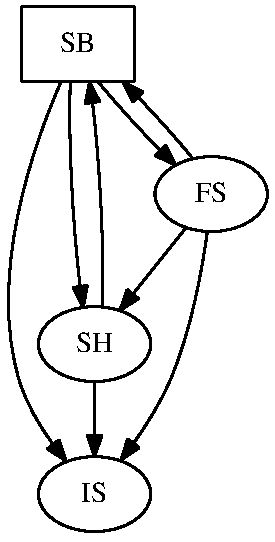
\includegraphics[scale=0.70]{trans_whole.pdf}}
  \caption{Mode transitions with states SB to SH, FS and IS}
  \label{fig:trans_whole}
\end{figure}

From the initial set of properties, it seems difficult to be able to remove some. We could add new ones,
but it would need to be interesting from a system standpoint. For example we might want to prove that 
the OBU is \emph{never} in isolated mode if not requested by the driver. We could write this as:

$$(SB\rightarrow IS) \lor (SH\rightarrow IS) \lor (FS\rightarrow IS) \implies Isolated\_by\_Driver$$

We could also state that the IS state is a ``dead'' state (state with no exits). This provides the 
following, for the subset of modes provided here.

$$\lnot((IS \rightarrow FS) \lor (IS \rightarrow SB) \lor (IS \rightarrow SH))$$

This is of course redundant with the previous properties the state machine, but it provides a 
simple and understandable safety property that cover exactly the safety need.

We could try to do the same for the other modes, but it will be the same problem. Most of the safety 
behavior is yielded by the model itself and it is difficult to produce a set of
declarative properties, and to avoid paraphrase. Nevertheless, it is useful to point out some specific 
and important system properties, even if they are not sufficient to capture the whole behavior of 
the state machine. In this case, these properties must come on top of the mere rephrase of the model.

Of course, it would also be possible to switch to a ```bigger scale'' view, and state properties
directly from the transition conditions to the behaviors allowed in the mode, but these properties 
would probably be difficult to prove without the intermediate layer provided by the modes themselves.
And as far as modularity is considered, the properties and proofs would be difficult to maintain in 
case of evolution of the system.


\section{Conclusion}
The two examples studied (establishment of the communication and mode transitions) are not exhaustive
in order to determine what would be the best formal language for safety properties (for this purpose
it would be useful to study also the braking curves and the MA), but they are sufficient to outline 
the upper part (or ``system'' part) of the process that would be necessary in order to prove safety 
in the context of OpenETCS: it starts by determining what is Vital and Non Vital, and by going down 
from the higher level safety properties to the model level safety properties. A synthetic view of the
process is presented on Fig. \ref{fig:saf_process}

On these two examples, we have seen that in some cases, it only needs a few safety properties to capture
the full safety behavior of the function, while in other cases, the full state machine (or a rephrase of 
it) is necessary. We have also seen than in the latter, it can also be useful to provide safety 
properties to express a particularly interesting (or sensitive) point.

In both case, the safety properties provide the backbone of the safety analysis. Writing them down 
allow to enhance knowledge and comprehension of the system, and they may also be used as Proof 
Obligations, as assertion to check when the model is running, or even in order to provide help in the
generation (manual or automatic) of test cases. 

\begin{figure}
  \centering
  \fbox{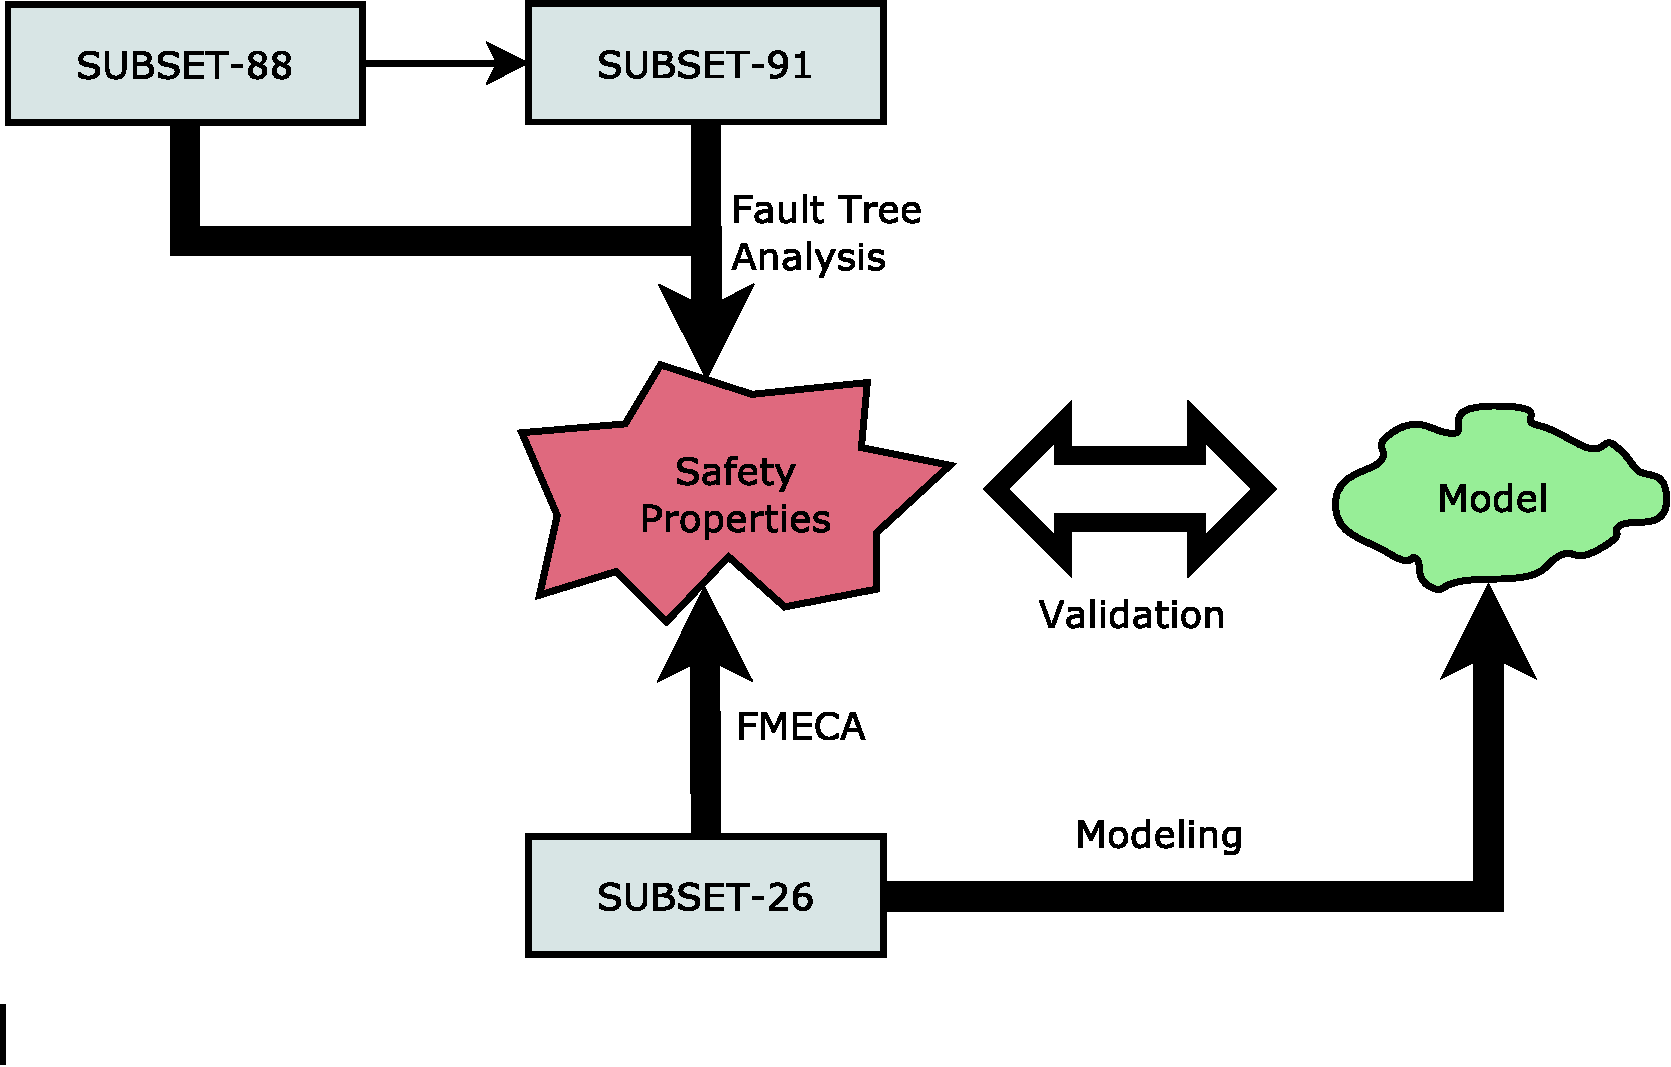
\includegraphics[scale=0.50]{process.pdf}}
  \caption{Outline of the safety analysis process}
  \label{fig:saf_process}
\end{figure}

\end{document}